\documentclass[tikz,border=2pt]{standalone}
\usepackage[T1]{fontenc}
\usepackage[utf8]{inputenc}
\usepackage{amsmath,amssymb}

% ACM
%\usepackage[tt=false, type1=true]{libertine}
%\usepackage[varqu]{zi4}
%\usepackage[libertine]{newtxmath}

% IEEE
\renewcommand{\sfdefault}{phv}
\renewcommand{\rmdefault}{ppl}
\renewcommand{\ttdefault}{pcr}
\usepackage{mathptmx}

\usepackage{pgfplots}
\pgfplotsset{compat=1.18}
\usepgfplotslibrary{groupplots}
\usepgfplotslibrary{colormaps}
\tikzset{
	fill-color/.style={
		color of colormap={#1},
		draw=.!80!black,
		fill=.!80!white,
	},
	normal-color/.style={
		color of colormap={#1},
		draw=.,
	},
	mydashed/.style={dash pattern=on 6pt off 4pt}
}

\makeatletter
\pgfplotsset{
	groupplot xlabel/.initial={},
	every groupplot x label/.style={
		at={($({\pgfplots@group@name\space c1r\pgfplots@group@rows.west}|-{\pgfplots@group@name\space c1r\pgfplots@group@rows.outer south})!0.5!({\pgfplots@group@name\space c\pgfplots@group@columns r\pgfplots@group@rows.east}|-{\pgfplots@group@name\space c\pgfplots@group@columns r\pgfplots@group@rows.outer south})$)},
		yshift=2ex,
		anchor=north,
	},
	groupplot ylabel/.initial={},
	every groupplot y label/.style={
		rotate=90,
		at={($({\pgfplots@group@name\space c1r1.north}-|{\pgfplots@group@name\space c1r1.outer
				west})!0.5!({\pgfplots@group@name\space c1r\pgfplots@group@rows.south}-|{\pgfplots@group@name\space c1r\pgfplots@group@rows.outer west})$)},
		anchor=south
	},
	execute at end groupplot/.code={%
		\node [/pgfplots/every groupplot x label]
		{\pgfkeysvalueof{/pgfplots/groupplot xlabel}};  
		\node [/pgfplots/every groupplot y label] 
		{\pgfkeysvalueof{/pgfplots/groupplot ylabel}};  
	}
}

\def\endpgfplots@environment@groupplot{%
	\endpgfplots@environment@opt%
	\pgfkeys{/pgfplots/execute at end groupplot}%
	\endgroup%
}
\makeatother

% Code from Christian Feuersänger
% https://tex.stackexchange.com/questions/54794/using-a-pgfplots-style-legend-in-a-plain-old-tikzpicture#54834

% argument #1: any options
\newenvironment{customlegend}[1][]{%
	\begingroup
	% inits/clears the lists (which might be populated from previous
	% axes):
	\csname pgfplots@init@cleared@structures\endcsname
	\pgfplotsset{#1}%
}{%
	% draws the legend:
	\csname pgfplots@createlegend\endcsname
	\endgroup
}%

% makes \addlegendimage available (typically only available within an
% axis environment):
\def\addlegendimage{\csname pgfplots@addlegendimage\endcsname}


\begin{document}
% This file was created with tikzplotlib v0.10.1.
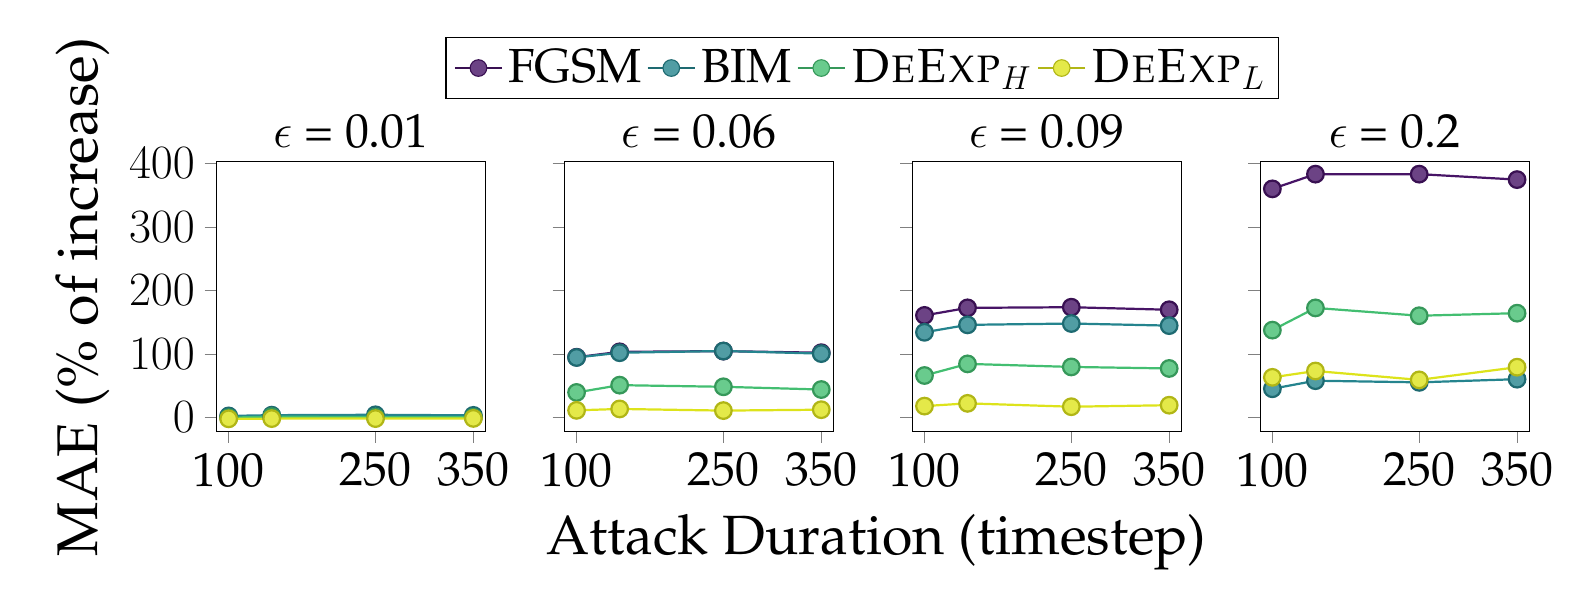
\begin{tikzpicture}

\definecolor{darkgray176}{RGB}{176,176,176}
\definecolor{green}{RGB}{0,128,0}
\definecolor{lightgray204}{RGB}{204,204,204}
\definecolor{purple}{RGB}{128,0,128}
\definecolor{yellow}{RGB}{255,255,0}

\begin{groupplot}[group style={group size=4 by 1},
	width=5cm, height = 5cm,
	xlabel style={font=\huge},
	ylabel style={font=\huge},
	xticklabel style={font=\LARGE},
	yticklabel style={font=\LARGE},
	title style={font=\LARGE,yshift=-1ex},
	groupplot xlabel = {\fontsize{20}{33} \selectfont Attack Duration (timestep)},
	xtick={100,250,350},
	xticklabels={100,250,350},
	yticklabel style={%
		scaled y ticks = false,
		/pgf/number format/.cd,
		fixed,
		precision=0,
		fixed zerofill,
		1000 sep={\,},
	},
	xticklabel style={%
		scaled y ticks = false,
		/pgf/number format/.cd,
		fixed,
		precision=0,
		fixed zerofill,
		1000 sep={\,},
	},colormap/viridis
	]
\nextgroupplot[
tick align=outside,
tick pos=left,
title={\(\displaystyle \epsilon\) = 0.01},
xmin=87.5, xmax=362.5,
ylabel={MAE (\% of increase)},
ymin=-21.78, ymax=402.38,
]
\addplot [thick, normal-color={50}, mark=*, mark size=3, mark options={solid,fill-color={50}}]
table {%
100 0.1
144 0.7
250 1.1
350 0.2
};
\addplot [thick, normal-color={450}, mark=*, mark size=3, mark options={solid,fill-color={450}}]
table {%
100 2.1
144 3.3
250 3.9
350 3
};
\addplot [thick, normal-color={700}, mark=*, mark size=3, mark options={solid,fill-color={700}}]
table {%
100 -0.7
144 1
250 0.2
350 0
};
\addplot [thick, normal-color={950}, mark=*, mark size=3, mark options={solid,fill-color={950}}]
table {%
100 -2.5
144 -2.1
250 -2.1
350 -1.8
};

\nextgroupplot[
scaled y ticks=manual:{}{\pgfmathparse{#1}},
tick align=outside,
tick pos=left,
title={\(\displaystyle \epsilon\) = 0.06},
x grid style={darkgray176},
xmin=87.5, xmax=362.5,
ymin=-21.78, ymax=402.38,
yticklabels={}
]
\addplot [thick, normal-color={50}, mark=*, mark size=3, mark options={solid,fill-color={50}}]
table {%
100 94.6
144 103.1
250 104.2
350 101.7
};
\addplot [thick, normal-color={450}, mark=*, mark size=3, mark options={solid,fill-color={450}}]
table {%
100 94.2
144 101.7
250 104.4
350 100.3
};
\addplot [thick, normal-color={700}, mark=*, mark size=3, mark options={solid,fill-color={700}}]
table {%
100 39.1
144 50.6
250 48
350 43.7
};
\addplot [thick, normal-color={950}, mark=*, mark size=3, mark options={solid,fill-color={950}}]
table {%
100 10.9
144 13.1
250 10.5
350 11.9
};

\nextgroupplot[
scaled y ticks=manual:{}{\pgfmathparse{#1}},
tick align=outside,
tick pos=left,
title={\(\displaystyle \epsilon\) = 0.09},
xmin=87.5, xmax=362.5,
ymin=-21.78, ymax=402.38,
yticklabels={}
]
\addplot [thick, normal-color={50}, mark=*, mark size=3, mark options={solid,fill-color={50}}]
table {%
100 160.5
144 172.4
250 173.4
350 169.4
};
\addplot [thick, normal-color={450}, mark=*, mark size=3, mark options={solid,fill-color={450}}]
table {%
100 133.9
144 145.6
250 147.7
350 144.4
};
\addplot [thick, normal-color={700}, mark=*, mark size=3, mark options={solid,fill-color={700}}]
table {%
100 65.8
144 84.1
250 79.3
350 76.9
};
\addplot [thick, normal-color={950}, mark=*, mark size=3, mark options={solid,fill-color={950}}]
table {%
100 17.6
144 21.9
250 16.6
350 19
};

\nextgroupplot[
scaled y ticks=manual:{}{\pgfmathparse{#1}},
tick align=outside,
tick pos=left,
title={\(\displaystyle \epsilon\) = 0.2},
xmin=87.5, xmax=362.5,
ymin=-21.78, ymax=402.38,
yticklabels={}
]
\addplot [thick, normal-color={50}, mark=*, mark size=3, mark options={solid,fill-color={50}}]
table {%
100 359.9
144 383.1
250 383.1
350 374.5
};
\addplot [thick, normal-color={450}, mark=*, mark size=3, mark options={solid,fill-color={450}}]
table {%
100 44.9
144 57.6
250 55
350 60
};
\addplot [thick, normal-color={700}, mark=*, mark size=3, mark options={solid,fill-color={700}}]
table {%
100 137.3
144 172.3
250 160
350 164
};
\addplot [thick, normal-color={950}, mark=*, mark size=3, mark options={solid,fill-color={950}}]
table {%
100 62.9
144 72.9
250 58.9
350 78.9
};
\end{groupplot}
\begin{customlegend}[colormap/viridis,
legend entries={ % <= in the following there are the entries
	FGSM,
	BIM,
	\textsc{DeExp}$_H$,
	\textsc{DeExp}$_L$,
},
legend columns=-1,
legend style={at={(13.5,5)},font=\LARGE}] % <= to define position and font legend
% the following are the "images" and numbers in the legend
\addlegendimage{fill-color={50}, mark=*, mark size=3, mark options={solid}}
\addlegendimage{fill-color={450}, mark=*, mark size=3, mark options={solid}}
\addlegendimage{fill-color={700}, mark=*, mark size=3, mark options={solid}}
\addlegendimage{fill-color={950}, mark=*, mark size=3, mark options={solid}}
\end{customlegend}
\end{tikzpicture}
\end{document}
